\documentclass{article}

\usepackage[]{amsmath} 
\usepackage[]{amsthm} 
\usepackage[]{amssymb} 

\usepackage[]{thmtools} 
\declaretheorem[style=definition, qed=$\diamondsuit$]{definition}
\declaretheorem[style=definition]{corollary}
\declaretheorem[style=definition, qed=$\spadesuit$]{example}
\declaretheorem[style=definition]{proposition}

\usepackage[]{microtype} 
\usepackage[]{enumitem} 
\usepackage[]{graphicx} 
\usepackage[]{subcaption} 
\usepackage[]{makeidx} 
\makeindex

\usepackage[backend=biber, style=alphabetic]{biblatex} 
\addbibresource{mat2000.bib}
\usepackage[]{url} 
\urlstyle{sf}

\usepackage[]{cleveref} 

\newcommand{\R}{\ensuremath{\mathbb{R}}}
\newcommand{\C}{\ensuremath{\mathbb{C}}}
\newcommand{\A}{\ensuremath{\mathbb{A}}}
\newcommand{\V}{\ensuremath{\mathbb{V}}}

\renewcommand{\P}{\ensuremath{\mathbb{P}}}

\DeclareMathOperator{\Col}{Col}
\DeclareMathOperator{\rank}{rank}
\DeclareMathOperator{\Bl}{Bl}
\title{Algebraic Surfaces}
\author{Ivar Haugal{\o}kken Stangeby}
\date{\textsc{MAT2000 - Spring 2016}}

\begin{document}
    \tableofcontents

    \section{Preliminaries}
    \label{sec:preliminaries}
    
    In algebraic geometry the central objects of study is the set of solutions
    to polynomial equations. Finding the zeros of, as an example, the quadratic
    equation
    \begin{equation}
        \notag
        ax^2 + bx + c = 0
    \end{equation}
    is something most people that have been exposed to elementary mathematics
    have done. Later on, one learns how to find the zeroes of more general
    functions, of either one or several variables over some general field of
    coefficients. This leads us to our first definition.

    \begin{definition}[Polynomial ring\index{polynomial ring} \cite{Pol16}]
        A \emph{polynomial ring} in $n$ variables over a field $K$ is the set
        of all functions on the form
        \begin{equation}
            \notag
            f(x_1, \ldots, x_n) = \sum^{}_{\alpha} p_{\alpha}\prod_{i=1}^{n} x_n^{\alpha_i}
        \end{equation}
        where $\alpha = (\alpha_1, \alpha_2, \ldots, \alpha_n)$ is a
        multi-index, and $p_\alpha = p_{\alpha_1,\ldots,\alpha_n}$ is an
        element in $K$.  We denote this polynomial ring $K[x_1, x_2, \ldots,
        x_n]$.
    \end{definition} 
    As an example, the most familiar polynomial ring is $\R[x]$. Elements of
    this ring include
    \begin{align*}
        f_1(x) = x^2, && f_2(x) = \pi, && f_3(x) = x^{17} + x^{3} - e^{4}, && f_4(x) = x^2 + 1.
    \end{align*} 
    Note that some of these have zeroes in the real numbers $\R$ while some
    does not. Most notably is the function $f_4$ whose zeroes lie in the realm
    of complex numbers, $\C$.

    Given a set of polynomials, $f_1, f_2, \ldots, f_m$ in a polynomial ring
    $K[x_1, x_2, \ldots, x_n]$ we can look at their common zeroes. It is in our
    interest to restrict our attention to polynomial rings where the field of
    coefficients is algebraically closed. We recall the definition:

    \begin{definition}[Algebraically closed field {\cite[p.~287]{FK03}}\index{algebraically closed field}]
        A field $K$ is \emph{algebraically closed} if every non-constant
        polynomial in $K[x_1, x_2, \ldots, x_n]$ has a zero in $K$.
    \end{definition}
    Given an algebraically closed field $K$, we define \emph{affine
    $n$-space}\index{affine $n$-space} over $K$ to be the set of all
    $n$-tuples of elements of $K$. We denote affine $n$-space by $\A_K^n$ or
    $\A^n$ if the field of coefficients is clear from context.  For our intents
    and purposes, we will be working over the algebraically closed field of
    complex numbers $\C$. 
    
    We now define the mathematical object that is of utmost importance in the
    study of zeroes of polynomials, namely the variety.
    \begin{definition}[Affine algebraic variety {\cite[p.~3]{Har77}}\index{affine algebraic variety}]
        Given a set of polynomials $f_1, f_2, \ldots, f_m$ from a ring of
        polynomials, the set of points $(x_1, x_2, \ldots, x_n)$ in the affine
        space $\A_K^n$ that satisfy
        \begin{equation}
            \notag
            f_i(x_1, x_2, \ldots, x_n) = 0 \quad \text{for } i = 1, 2, \ldots, m
        \end{equation}
        is called an \emph{affine algebraic variety} and is denoted $\V(f_1,
        f_2, \ldots, f_m)$.
    \end{definition}

    Given the polynomial $f(x) = x^2 - 1$, the affine algebraic variety $\V(f)$
    is then the set $\left\{ 1, -1 \right\}$ since $f(1) = f(-1) = 0$. Given an
    additional polynomial $g(x) = x-1$ we have $\V(f, g) = \left\{ 1 \right\}$
    since $g(1) = 0$, but $g(-1) \neq 0$. Finally, if we also consider the
    polynomial $h(x) = x^2$, then $\V(f, g, h) = \emptyset$. We see as a simple
    fact, and state without proof the following.
    
    \begin{corollary}
        Given a set of polynomials $f_1, f_2, \ldots, f_m$, the variety
        $\V(f_1, f_2, \ldots, f_m)$ can be expressed as a finite intersection
        \begin{equation}
            \notag
            \V(f_1, \ldots, f_m) = \bigcap_{i=1}^{m} \V(f_i).
        \end{equation}
    \end{corollary}
    It is also of interest, especially when aiming to create and visualize
    interesting figures, that the following hold:
    \begin{corollary}
    Given a set of polynomials $f_1, f_2, \ldots, f_m$, the affine algebraic
    variety of the product $f_1f_2\cdots f_m$ is expressible as a finite union
    \begin{equation}
        \notag
        \V(f_1f_2\cdots f_m) = \bigcup_{i=1}^{m} \V(f_i).
    \end{equation}
    \end{corollary}
    
    With this in mind, we define one of the more interesting properties of
    varieties, and one we will work with a lot in this article, namely the
    singularities.
    \begin{definition}[Singularity {\cite[p.~3]{Whi08}}\index{singularity}]
        A singularity of the variety $V = \V(f_1, f_2, \ldots, f_m) \subset
        \A_K^n$ is a point $p \in V$ such that the Jacobian matrix
        \begin{equation}
            \notag
            A = \begin{bmatrix}
                \frac{\partial f_1}{\partial x_1} & \hdots & \frac{\partial f_1}{\partial x_n} \\
                \vdots & \ddots & \vdots \\
                \frac{\partial f_m}{\partial x_1} & \hdots & \frac{\partial f_m}{\partial x_n}
            \end{bmatrix}(p)
        \end{equation}
        has rank strictly less than $\min(m, n)$.
    \end{definition}

    A very useful consequence of this definition deal with the varieties of
    single polynomials and will aid us tremendously in the search for
    singularities.
    \begin{corollary}
        \label{crl:single_poly}
        A point $p$ is a singularity of the variety $V = \V(f) \subset \A_K^n$
        if and only if the partial derivatives of $f$ vanish identically at
        $p$. 
    \end{corollary}
    \begin{proof}
        We recall that the rank of a matrix is the dimension of its column
        space, that is for a matrix $A$, $\rank(A) = \dim(\Col(A))$.  Assume
        first that $p$ is a singularity of $V$. Then $\rank(A) < min(n, m) =
        1$. This means that the matrix $A$ has no independent columns,
        otherwise the columns of $A$ would span a space of dimension greater
        than or equal to one. The Jacobian matrix reads in this case
        \begin{equation}
            \notag
            A = \begin{bmatrix}
                \frac{\partial f}{\partial x_1}(p) & \hdots & \frac{\partial f}{\partial x_n}(p)
            \end{bmatrix}.
        \end{equation}
        Since the matrix has no independent columns, we cannot have any pivot
        columns, hence each entry must be zero. Consequently, all partial
        derivatives of $f$ vanish at $p$.  For the opposite implication, assume
        that the partials vanish identically at $p$. Then the Jacobian matrix
        reads
        \begin{equation}
            \notag
            A = \begin{bmatrix}
                0 & \hdots & 0
            \end{bmatrix},
        \end{equation} and consequently $A$ has rank strictly less than one.
        Hence $p$ is a point of singularity of $V$.
    \end{proof}

    We now have the tools needed to start looking at algebraic surfaces.
    
    \section{Algebraic Surfaces}
    \label{sec:algebraic_surfaces}
    
    In this section, we try to motivate the definition of an algebraic surface,
    and look at some examples. Hopefully, this will give an intuitive
    introduction to exactly what we will we looking at. We start by looking at
    real algebraic curves, as a good entry point.

    \subsection{Algebraic Curves}
    \label{sub:algebraic_curves}
    
    From elementary mathematics, one learns about real valued functions,
    $f(x)$, and how to plot these functions by setting $y = f(x)$ and plotting
    points in the $(x, y)$-plane. This yields a curve of sorts, moving around
    in the plane.

    The graph of a function is something of a peculiarity, because it comes
    with some restrictions. Not all curves in the $(x, y)$-plane correspond to
    a specific function. One of the standard methods for verifying whether a
    certain curve corresponds to a function or not, typically taught in school,
    is the \emph{vertical line test}. If you can draw a vertical line through
    two or more points on the curve, then the curve is not associated to any
    specific function. There is however a limit to how interesting
    function-curves can be.

    Having an equation $y = f(x)$ we can form the \emph{equation of a curve at
    zero}. We define a new function in two variables and equate it to zero.
    This yields
    \begin{equation}
        \notag
        g(x, y) = y - f(x) = 0.
    \end{equation}
    The set of points along the curve described by this equation is precisely
    the points that lie in the variety $\V(g(x, y))$.
    If the function $f(x)$ is a polynomial in the variable $x$, i.e., $f(x) \in
    K[x]$, we call the function curve of $f(x)$ algebraic. If the distinction
    between a function graph and curves is to be justified, then there has to
    be curves that are not function graphs.

    Plotting the result when setting $y^2 - x^3$, the plotted curve does not
    pass the vertical line test and is therefore something different from a
    function graph. Similarity, the equation $y^2 = x^3 + x^2$ defines another
    curve that is not a function graph. These are shown in
    \cref{fig:algebraic_curves}, and are prime examples of curves that exhibit
    a singularity. We will get back to the curve shown in \cref{fig:node}
    later.

    \begin{figure}[h!]
        \centering
        \begin{subfigure}[t]{0.45\textwidth}
            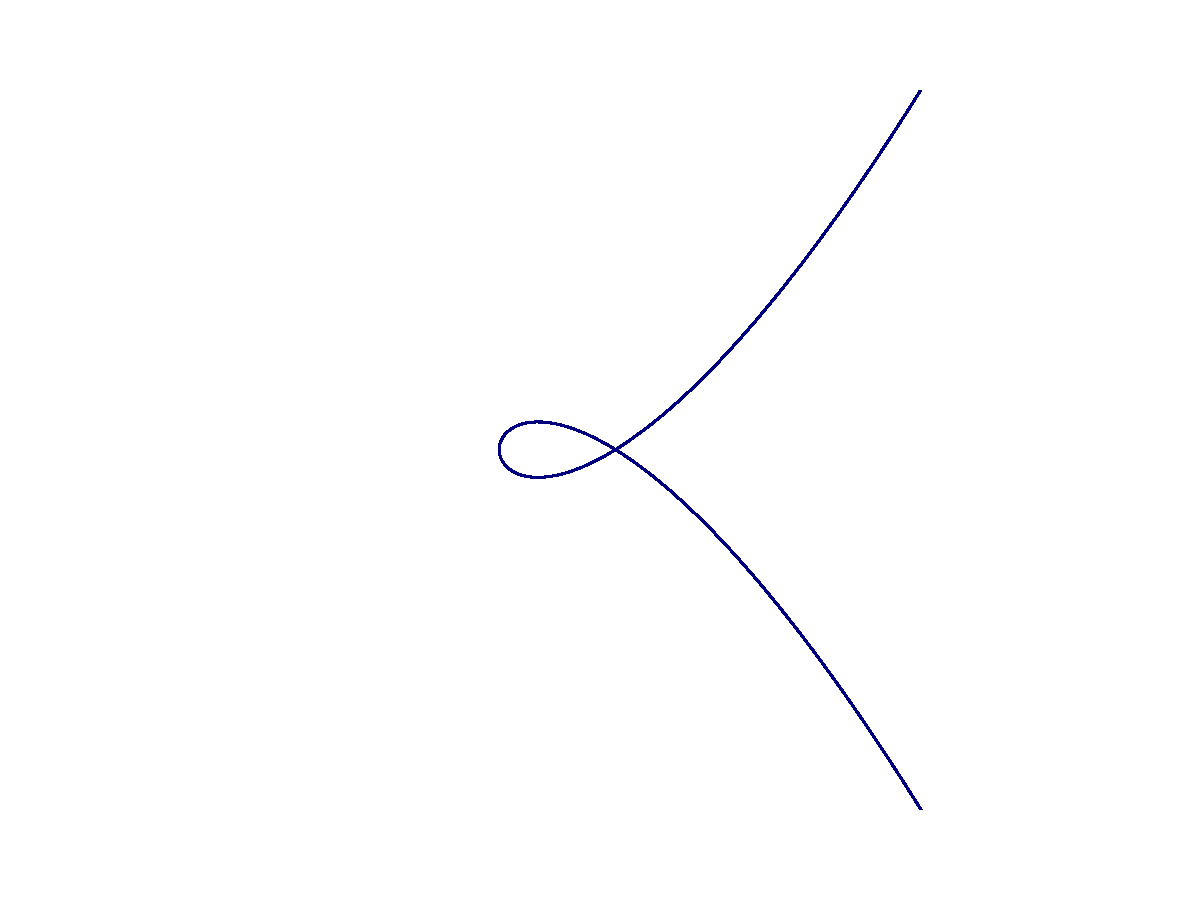
\includegraphics[width=\textwidth]{pictures/node.pdf}
            \caption{The curve given by the equation $y^2 - x^3 - x^2 = 0$.
            This curve is commonly known as ''The Node''. It exhibits a
            singularity at the point $p = (0, 0)$ which can be verified by
            computing the partial derivatives at $p$.}
            \label{fig:node}
        \end{subfigure}        
        ~
        \begin{subfigure}[t]{0.45\textwidth}
            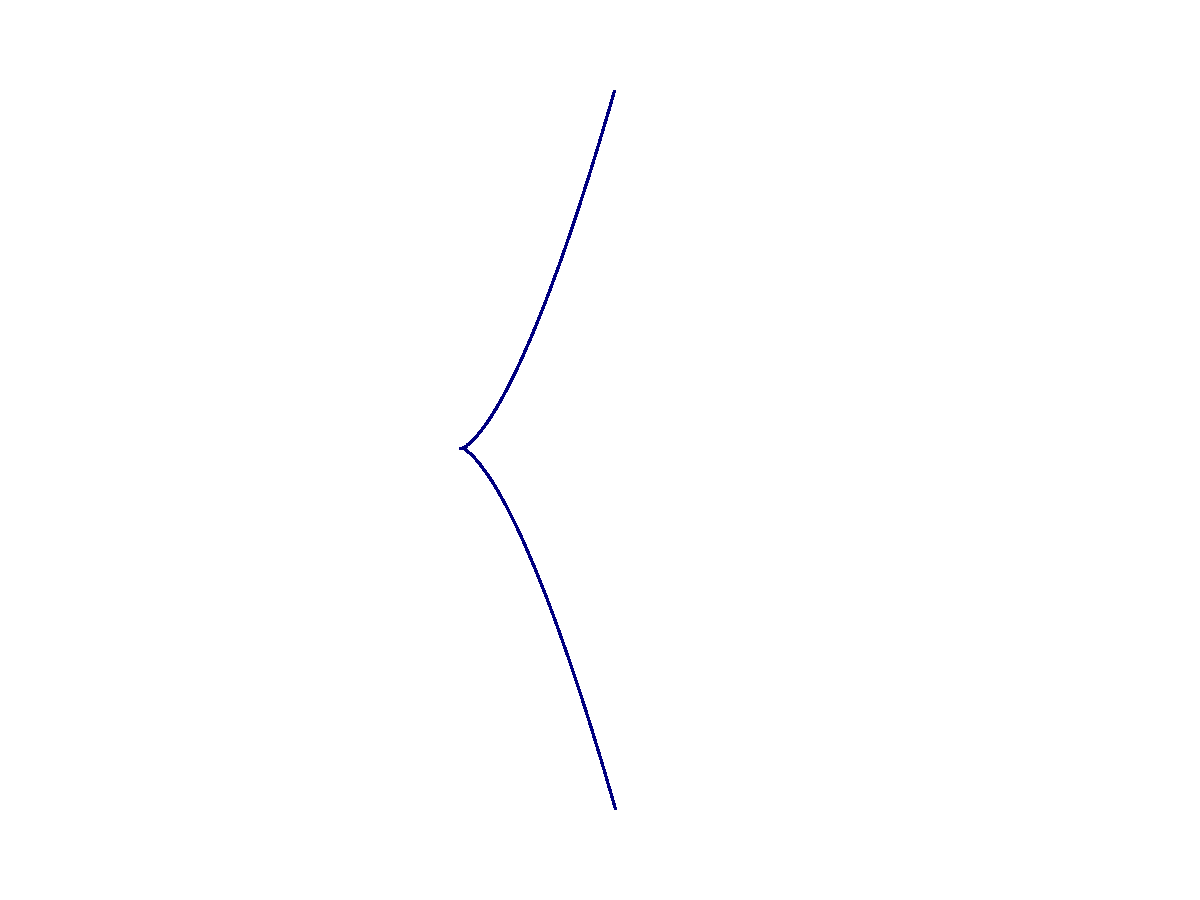
\includegraphics[width=\textwidth]{pictures/cusp.pdf}
            \caption{The curve given by $y^2 - x^3 = 0$, or more commonly known
            as ''The Cusp'', is also an example of a singular algebraic curve.
        The point $p = (0, 0)$ is a point of singularity.}
        \end{subfigure}
        \caption{Curves not corresponding to functions.}
        \label{fig:algebraic_curves}
    \end{figure}
    
    \subsection{Moving up a dimension}
    \label{sub:moving_up_a_dimension}
    With what we have done so far, we can generalize and move up a dimension.
    Instead of considering curves in the $(x, y)$-plane, we can instead look at
    surfaces in the three-dimensional $(x, y, z)$-space. Following the same
    procedure as above, we define a new function $h(x, y, z) = z - g(x, y)$.
    Completely analogous to the definition made for curves, we call the surface
    \emph{algebraic} if $h(x, y, z)$ is a polynomial in the variables $x, y,
    z$. That is $h(x, y, z) \in K[x, y, z]$. We give some examples.

    \begin{example}
        \label{exmpl:algebraic_surfaces}
        The following equations satisfy the definition of an algebraic surface:
        \begin{enumerate}
            \item $h_1(x, y, z) = z - xy = 0$,
            \item $h_2(x, y, z) = z - x^2 - y^2 = 0$,
            \item $h_3(x, y, z) = z - (2x^2 - y)(y - x^2) = 0$,
        \end{enumerate}
        while the following does \emph{not}:
        \begin{enumerate}[resume]
            \item $g_1(x, y, z) = \sin(xy) + z = 0$, and
            \item $g_2(x, y, z) = \tan^2(x) + \pi z y$.
        \end{enumerate}
        These examples are visualized in \cref{fig:algebraic_surfaces}.
        \begin{figure}[]
            \centering
            \begin{subfigure}[t]{0.3\textwidth}
                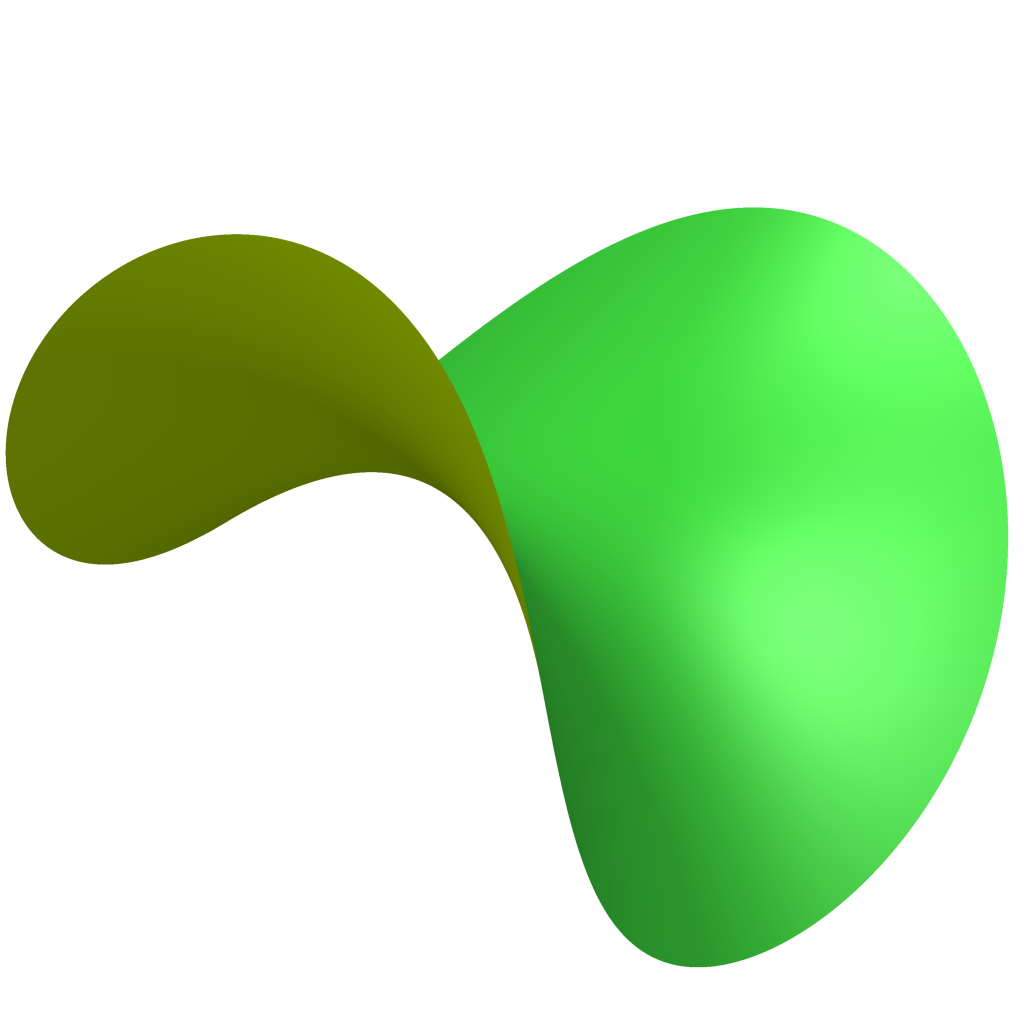
\includegraphics[height=0.6\textwidth]{pictures/example_one.png} 
                \caption{$h_1(x, y, z) = 0$}
            \end{subfigure}
            ~
            \begin{subfigure}[t]{0.3\textwidth}
                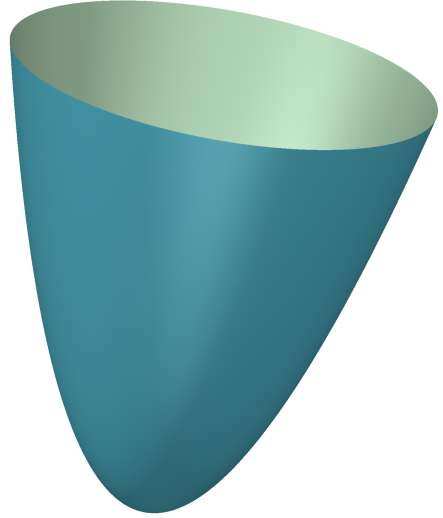
\includegraphics[height=0.6\textwidth]{pictures/example_two.png} 
                \caption{$h_2(x, y, z) = 0$}
            \end{subfigure}
            ~
            \begin{subfigure}[t]{0.3\textwidth}
                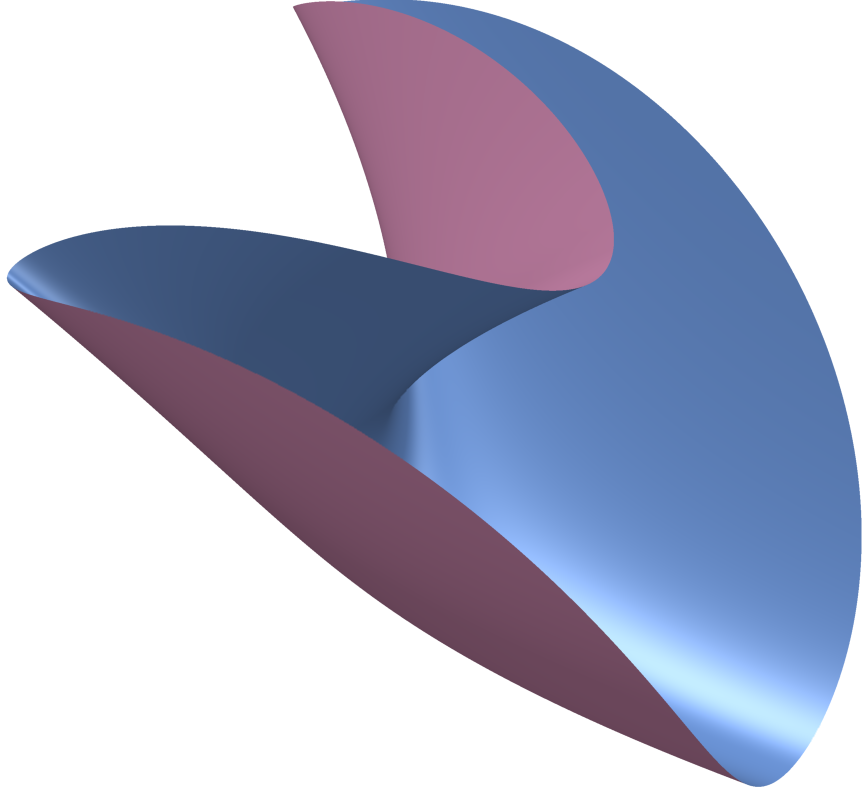
\includegraphics[height=0.6\textwidth]{pictures/example_three.png} 
                \caption{$h_3(x, y, z) = 0$}
            \end{subfigure}
            \caption{The surfaces that fell under the category algebraic from
            \cref{exmpl:algebraic_surfaces}.}
            \label{fig:algebraic_surfaces}
        \end{figure}
    \end{example}
    We can of course continue this process of introducing new functions and
    move up a dimension for each time indefinitely.  We complete this section
    by formally defining an algebraic surface. In any case, the surfaces are
    defined by the variety of some defining polynomial.
    \begin{definition}[Algebraic surface\index{algebraic surface}]
        An \emph{algebraic surface} is an algebraic variety of
        dimension\footnote{The dimension of an algebraic variety is a bit hard
            to grasp, and since we only will be dealing with algebraic surfaces
            in this text we do not spend any time classifying the different
        kinds of varieties. The explanation of this is therefore omitted. See
    \cite{Dim16}.}
            two.  We define the \emph{degree}\index{algebraic surface!degree}
            of an algebraic surface to be the highest combined power in the
            defining polynomials terms, and denote this $d$.  That is,
        \begin{equation}
            \notag
            d = \max_{\alpha}\left\{ \alpha_1 + \alpha_2 + \ldots \alpha_n \right\}
        \end{equation}
        where $\alpha_i$ is the power of $x_i$ in a term.
    \end{definition}
    We now take a brief look at some of the properties of these surfaces in
    relation to the singularities.
    
    \section{Singularities}
    \label{sec:singularities}
    The singularities of an algebraic surface is one of the important elements
    that give the surface its visual appeal. I am sure most people agree with
    me, when I say that a surface full of singularities is more intriguing than
    one with no singularities at all. The singularities, along with their
    configurations, symmetries and their number are things that one can explore
    further.
     
    \subsection{The number of singularities}
    \label{sub:the_number_of_singularities}

    For an algebraic surface of degree $d$ we let
    $\mu(d)$\index{singularity!$\mu(d)$, maximal number} denote the maximal
    number of singularities such a surface can have.  Determining $\mu(d)$ for
    even relatively small $d$ has proven to be surprisingly difficult.
    \cite{Lab14} gives a very intuitive introduction to the world of
    singularity-hunting and the search for the largest possible $\mu(d)$. We
    shall repeat some of the results here. We start with a non-example of a
    singular surface.
    
    \begin{proposition}[Singularities of the plane]
        Let $V = \V(f(x, y, z)) = \V(ax + by + cz + d)$ be a plane, then $V$ contains no
        singular points.
    \end{proposition} 
    \begin{proof}
        Assume for contradiction that $p \in V$ is a singular point. Then the
        Jacobian matrix of $ax + by + cz + d$ evaluated at $p$ must have rank
        strictly less than 1, or equivalently, by \cref{crl:single_poly}, the
        partial derivatives vanish at $p$. The partial derivatives of our
        defining polynomial is given by
        \begin{align*}
            \notag
            \frac{\partial f}{\partial x} = a, && \frac{\partial f}{\partial y} = b, &&  \frac{\partial f}{\partial z} = c,
        \end{align*}
        however, none of these are dependent on the point we chose. Hence, for
        these partials to vanish at $p$, we need $a = b = c = 0$. However, our
        variety $V$ then reduces to $\V(d)$ where $d$ is some constant. If $d
        \neq 0$, then $\V(d) = \emptyset$, and therefore does not contain $p$
        at all, which contradicts our assumption. If $d = 0$ on the other hand,
        then we are left with the equation $0 = 0$ which does not describe a
        plane. Consequently, $p$ cannot be a singular point of $V$, and the
        plane therefore exhibits no singularities. 
    \end{proof}
    The argument above tells us that for a general algebraic surface of degree
    $d = 1$, we can have no singularities, hence $\mu(1) = 0$.

    We now look at a surface with four singularities.
    \begin{example}[The Cayley cubic\index{the cayley cubic}]
        The Cayley cubic, a surface of degree $d = 3$, is defined by the
        polynomial
        \begin{equation}
            f(x, y, z) = xyz + (1 - x - y - z)(yz + xz + xy).
        \end{equation}
        We are interested in finding the singularities of this surface, if there are any.
        We first compute the partial derivatives and find that
        \begin{align*}
            \frac{\partial f}{\partial x} &= -(y + z)(2x + y + z - 1), \\
            \frac{\partial f}{\partial y} &= -(x + z)(x + 2y + z - 1), \\
            \frac{\partial f}{\partial z} &= -(x + y)(x + y + 2z - 1).
        \end{align*}
        By inspection, we see that the three partials vanish in the point $(1,
        0, 0)$. Due to the symmetric nature\footnote{The study of symmetric
        functions\index{symmetric function} are also of great interest, which
        we will not go into detail here. However, as a brief mention, given a
        function $f(x_1, x_2, \ldots, x_n)$ and a permutation $\sigma \in S_n$,
        where $S_n$ is the symmetry group on $n$ letters, one can consider the
        set $\mathcal{S} = \left\{ \sigma \in S_n \mid f\left(x_{\sigma(1)},
        x_{\sigma(2)}, \ldots, x_{\sigma(n)}) = f(x_1, x_2, \ldots,
        x_n\right)\right\}$ of permutations that fixes the function $f$. For
        the Cayley cubic discussed above, any $\sigma \in S_3$
        fixes the function, and hence the zeros were easily found by symmetry.} of the
        defining equation, we see that $(0, 1, 0)$ and $(0, 0, 1)$ also are zeroes of
        these polynomials.  Finally, the partials also vanish in the point $(0, 0, 0)$.
        We also see that $f(1, 0, 0) = f(0, 1, 0) = f(0, 0, 1) = f(0, 0, 0) = 0$ so
        these are indeed singularities of the Cayley cubic. The symmetries in the
        defining polynomial is seen reflected in the visualized surface shown in
        \cref{fig:cayley}.

        \begin{figure}[h!]
            \centering
            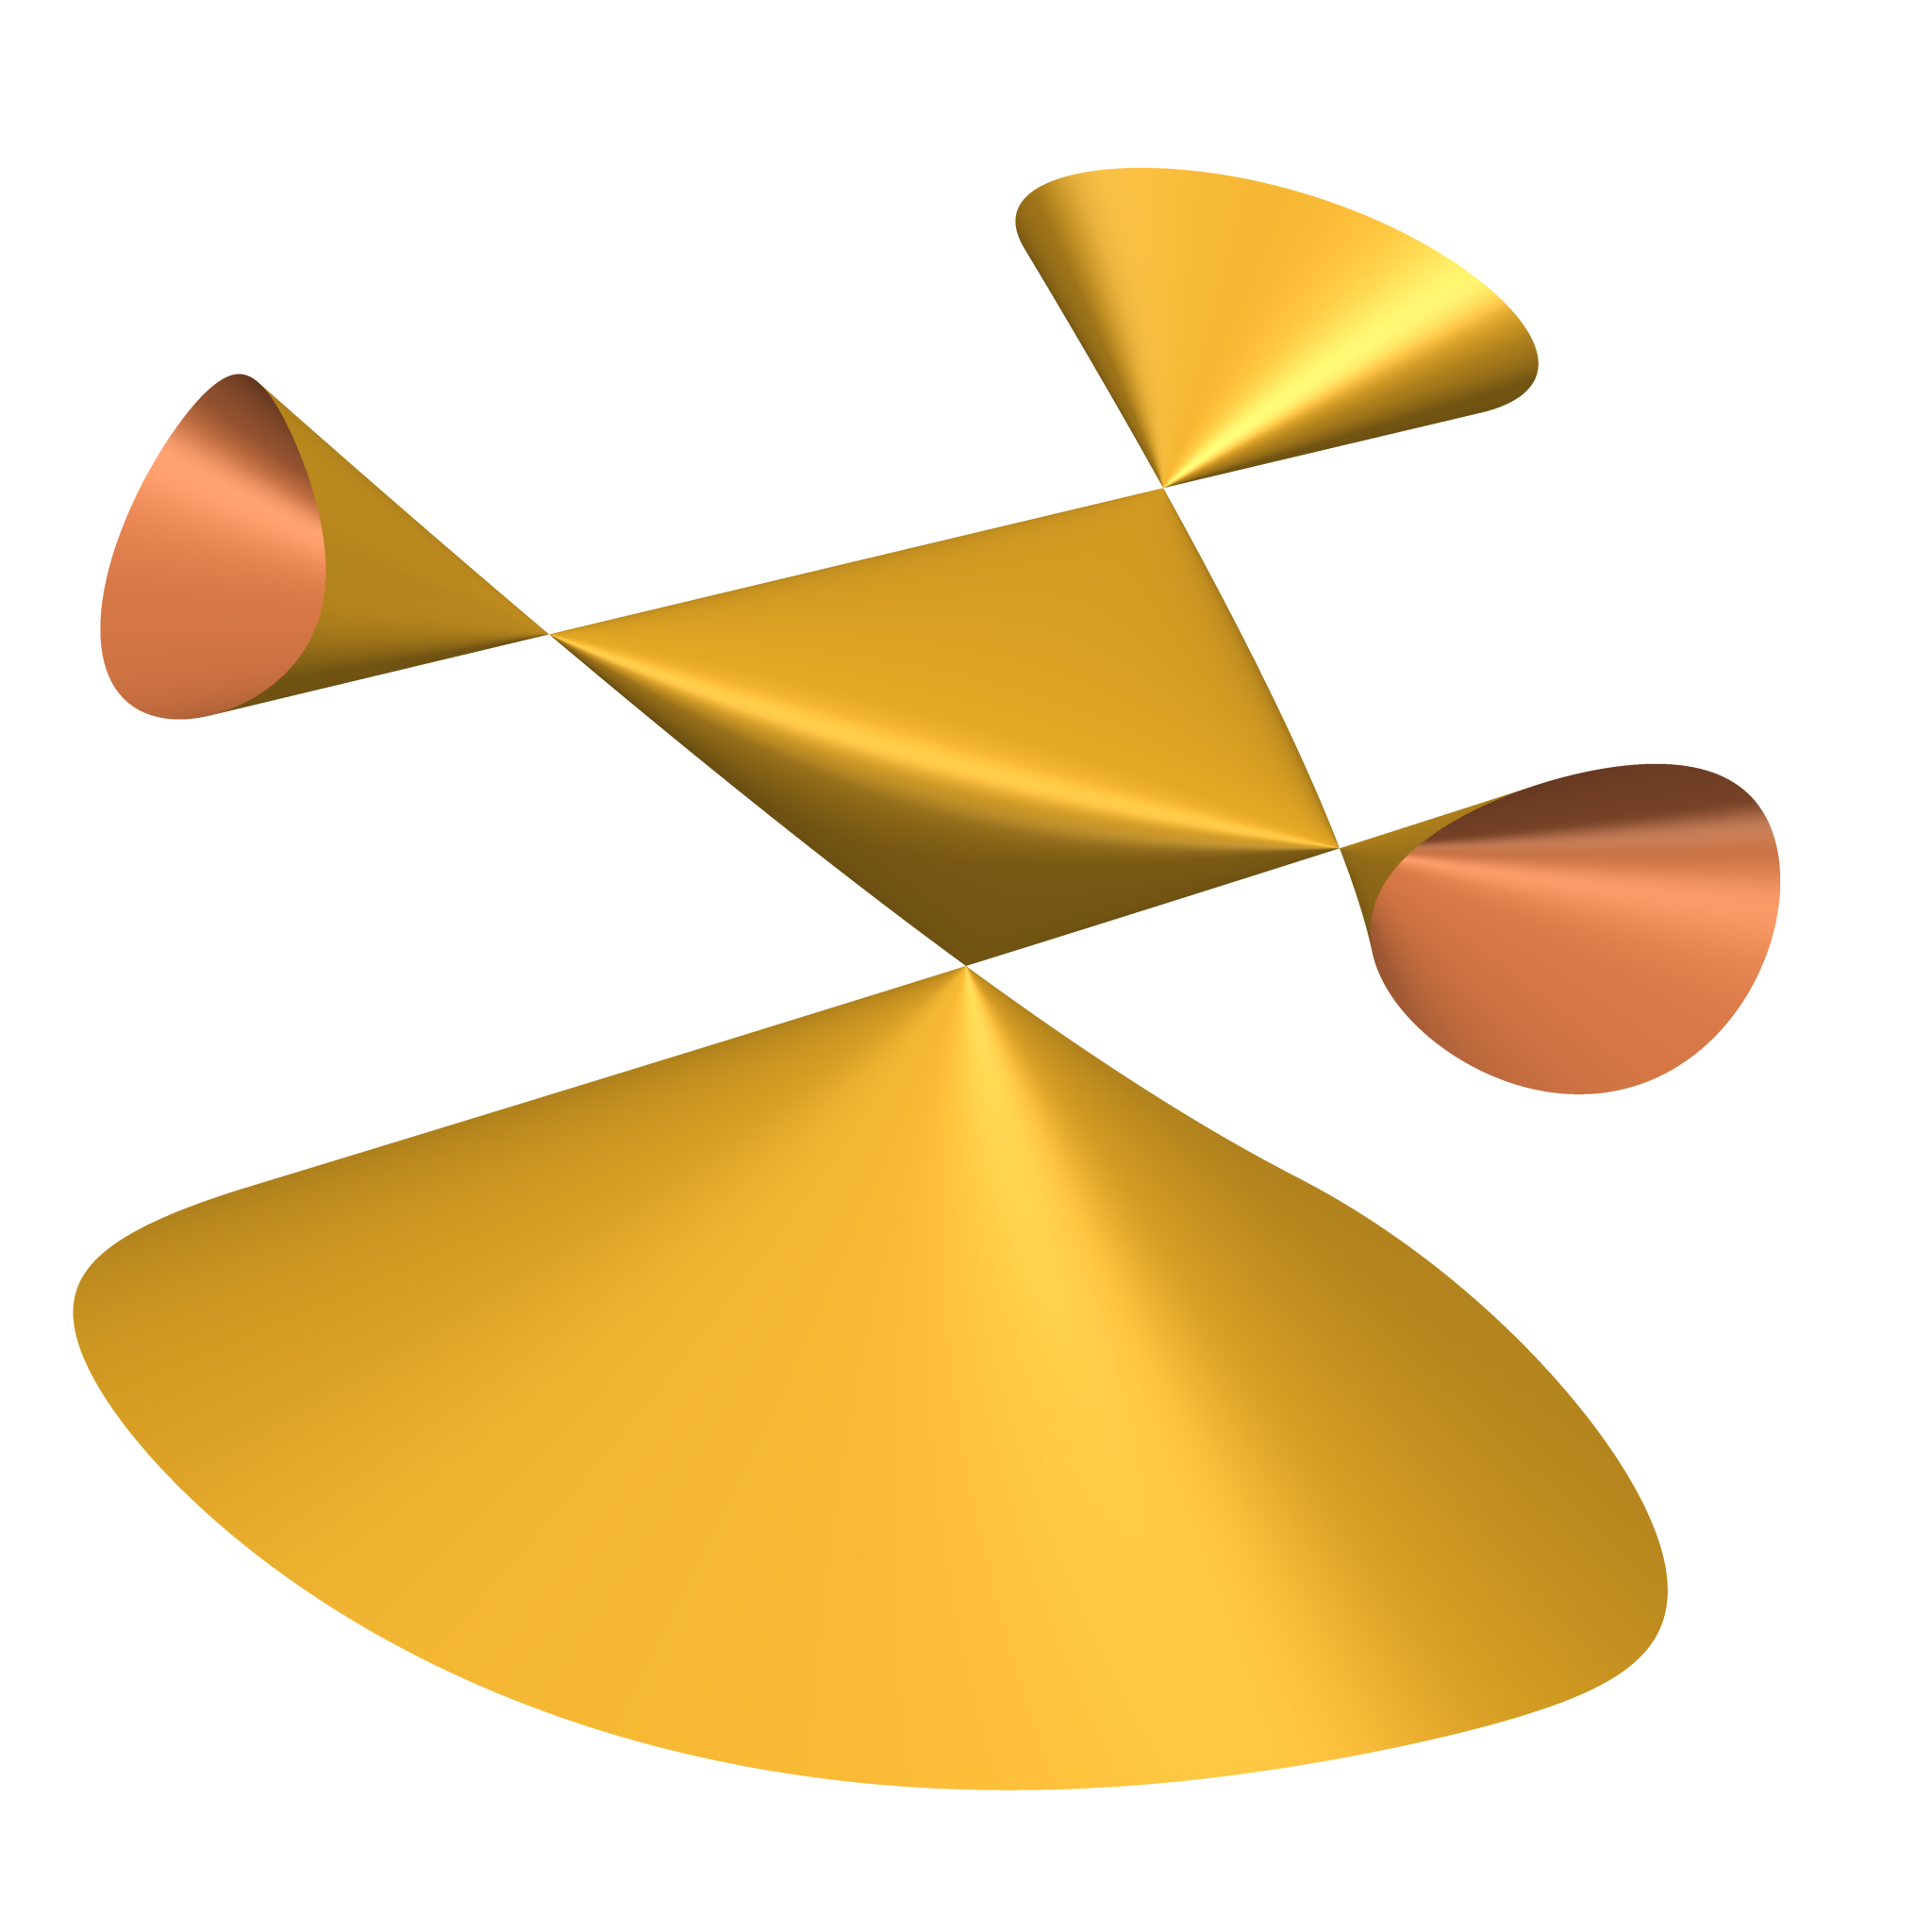
\includegraphics[width=0.3\linewidth]{pictures/cayley_cubic.png}
            \caption{The Cayley cubic, a degree three surface given by the
                equation $f(x, y, z) = xyz + (1 - x  - y - z)(yz + xz + xy)$.
                It is a good example of a surface whose set of singularities
                show a lot of symmetry. It also exhibit the maximal number of
                singularities for a degree $3$ surface, namely 4.}
            \label{fig:cayley}
        \end{figure}
    \end{example}     
    
    From \cite[p.~7]{Lab14} we have the following relation on the maximum
    number of singularities for $d \geq 3$,
    \begin{equation}
        \notag
        \mu(d) \leq \frac{1}{2}(d(d-1)^2 - 3)
    \end{equation}
    and plugging in $d = 3$ yields $\mu(d) \leq 4$. However, we have already
    presented a surface of degree $d = 3$ with four singularities, so in fact
    $\mu(d) = 4$. The theory of finding the maximal number of singularities of
    a given degree and constructing surfaces that exhibit all is a very
    technical matter. The thesis \cite{oliver2005hypersurfaces} gives a good
    introduction to the construction and visualization of such surfaces.

    We have now had a brief look at singularities of surfaces, and how to find
    them, we now consider how to remove, or \emph{resolve}, such singularities.
    
    \section{Resolving singularities}
    \label{sec:resolving_singularities}
    
    We call a variety that exhibits no singularities \emph{smooth}\index{smooth
    variety}. It is often possible to study a smooth copy of a variety with
    singularities if we move from affine space to projective space. This
    process can be defined in many different ways, with the seemingly most
    prevalent one being through maps from various spaces to each other. In this
    paper we will try to keep it as intuitive as possible, by using the more
    geometrically based procedure. We first define the notion of a projective
    space.

    \subsection{Projective space}
    \label{sub:projective_space}
    
    Informally, projective space generalizes the notion of parallel lines
    intersecting at infinity. The general definition of projective $n$-space is
    the set of lines in $\A^{n+1}$ passing through the origin. For our purposes
    we will take $\A^{n+1} = \C^{n+1}$.

    \begin{definition}[The projective space of dimension $n$\index{projective space}]
        Let $\sim$ be a relation on $\C^{n+1}\setminus \left\{ 0 \right\}$ defined by
        \begin{equation}
            \notag
            (x_1, \ldots, x_{n+1}) \sim (x_1', \ldots, x_{n+1}')
            \iff (x_1', \ldots, x_{n+1}') = \lambda(x_1, \ldots,
            x_{n+1})
        \end{equation}
        where $\lambda$ is some non-zero complex number. This relation can be
        shown to be an equivalence relation. We denote the
        equivalence class of $(x_1, x_2, \ldots, x_{n+1})$ by $\left[ x_1 : x_2
        : \ldots : x_{n+1} \right]$ and define the \emph{projective space of
        dimension $n$} as the set 
        \begin{equation}
            \notag
            \P^{n}_\C = \left\{ \left[ x_1 : \ldots : x_{n+1} \right] \mid (x_1,
            \ldots , x_{n+1}) \in \C^{n+1}\setminus \left\{ 0 \right\}\right\}.
        \end{equation}
        The elements in $\P_\C^n$ are called \emph{homogeneous
        coordinates}\index{homogeneous coordinates}. 
    \end{definition}

    We now turn to the resolution of singularities. There are, as mentioned
    above, many ways of doing this, but we will here apply a geometrical
    approach.

    \subsection{Blowing up a point singularity.}
    \label{sub:blowing_up_a_point_singularity_}
    
    We start by examining resolutions of single points. Informally, when we
    blow up a point $p$ in $\A^n$, we replace the point $p$ by an entire copy
    of a projective space $\P^{n-1}$ and try to leave the rest of the space
    $\A^n$ ''unchanged''. We will give a few examples, that hopefully will
    illustrate the geometrical aspect of this, but first a formal definition.

    \begin{definition}[Blowup of $\A^{n}$ at a point $p$.]
        We let the \emph{blowup-surface}\index{blowup-surface!in a point}
        $\Bl_p\A^{n}$ be the set of all pairs consisting of a point $p \in
        \A^n$ and a line from $p$ through the origin. The surface is embedded
        in the space $\A^n\times\P^{n-1}$. We write
        \begin{equation}
            \notag
            \Bl_p\A^n = \left\{ (p, L) \mid p \in \A^{n} \text{ and } p \in L \right\}.
        \end{equation}
    \end{definition}
    Now, this is a fairly technical definition, so where do we go from here?
    When blowing up a surface at a point $p$ we are essentially giving the
    surface ''more room'' so that the points creating the singularities can
    pass each other without hassle. In order to aid us with the above
    definition, we show the following claim that tells us under what
    circumstances the point $p$ lie on the line $L$:

    \begin{proposition}
        \label{prop:point_line}
        Given a point $x = (x_1, x_2, \ldots, x_n)$ in $\A^n$ and a point $y =
        [y_1 : y_2 : \ldots : y_n]$ in the space $\P^{n-1}$, the point $x$ is a
        multiple of $y$ if and only if the matrix
        \begin{equation}
            \notag
            A = \begin{bmatrix}
                x_1 & x_2 & \hdots & x_n \\
                y_1 & y_2 & \hdots & y_n
            \end{bmatrix}
        \end{equation}
        has rank less than or equal to one. Similarly, the rank is less than or
        equal to one only if each $2\times 2$-minor $x_iy_j - x_jy_i = 0$ for
        $1 \leq i < j \leq n$.
    \end{proposition} 
    \begin{proof}
        In order to verify this, we recall that $\rank(A) = \rank(A^T)$, so we
        chose to work with the transposed matrix instead. Assume that $x$ is a
        multiple of $y$, so $y = \lambda x$ for some scalar $\lambda$. Then
        \begin{equation}
            \notag
            A^T = \begin{bmatrix}
                x_1 \;\, \lambda x_1 \\
                x_2 \;\, \lambda x_2 \\
                \vdots \\
                x_n \;\, \lambda x_n
            \end{bmatrix}
        \end{equation}
        is the associated matrix. If $x = 0$, then $A^T$ is the zero matrix and
        has therefore rank 0. If $x \neq 0$, then we have exactly one pivot
        column in this matrix, hence $\dim(\Col(A^T)) = 1$. In any case,
        $\rank(A) = \rank(A^T) \leq 1$. For the opposite implication. If $A$
        has rank 0, then $A$ is the zero matrix, and hence trivially, $x$ is a
        multiple of $y$, both being zero. If $A$ has rank $1$, then there is
        one linearly independent column in $A^T$, hence the other column can be
        expressed as a multiple of the first. In other words, $x$ is a multiple
        of $y$.
        
        If there were a non-zero minor $r\times r$ for $r > 1$, then this
        suggests that there are $r$ linearly independent column vectors, but
        this can't occur since $\rank(A^T) \leq 1$.
    \end{proof}
    
    With the above result, we can rewrite the definition of the blowup-surface
    $\Bl_p\A^n$ as
    \begin{equation}
        \notag
        \Bl_p\A^n = \left\{ (x_1, x_2, \ldots, x_n; y_1 : y_2 : \ldots : y_n)
    \mid x_iy_j = x_jy_i \text{ for } 1 \leq i < j \leq n \right\}
    \end{equation} which is computationally easier to work with.

    We now give some examples of the computations involved when finding
    blowup-surfaces. We start with the resolution of a singularity in an
    algebraic curve.
    \begin{example}[The node]
        The Node, shown in \cref{fig:node}, is a singular algebraic curve with
        a singularity in the point $p = (0, 0)$. The defining polynomial of the
        node is given by
        \begin{equation}
            \label{eq:node}
            f(x, y) = y^2 - x^2 - x^3,
        \end{equation}
        with the curve $\mathcal{C} = \V(f(x, y, z))$. This curve lies in the
        affine plane $\A^2$, while the resulting blowup-surface of
        $\mathcal{C}$ at the point $(0, 0)$ lies in the space $\A^2 \times
        \P^1$. For a point $(x, y) \in \mathcal{C}$ we need to figure out what
        line passes through both $(x, y)$ and the origin $(0, 0)$. However,
        \cref{prop:point_line} tells us exactly under what circumstances this
        occurs. Let $[u : v]$ be a point in $\P^1$. Then, the matrix
        \begin{equation}
            \notag
            A = \begin{bmatrix}
                x & y \\
                u & v
            \end{bmatrix}
        \end{equation}
        has rank less than or equal to one only when $xv - yu = 0$, our only
        $2\times 2$-minor in this case. This gives us the equation $xv = yu$.
        We chose the point $(u, v)$ as a representative for the equivalence
        class $[u : v]$ however, we might as well chose the point $(u, 1)$ or
        $(1, v)$, since we can set either $u = 1$ or $v = 1$ and then multiply
        the representative by $1 / u$ or $1 / v$ respectively. This makes us
        able to eliminate either $u$ or $v$ from $xv = yu$. This gives us two
        different cases:
    
        \paragraph{Case 1:}
        \label{par:case_1}
        
        Setting $u = 1$ we get the equation $y = xv$. This can be substituted
        back into \cref{eq:node} in order to eliminate $y$. This gives us a new
        equation, namely
        \begin{equation}
            \notag
            g(x, v) = x^2(v^2 - 1 - x).
        \end{equation}
        This function $g(x, v)$ is what we call an \emph{affine
        chart}\index{affine chart} of the blowup-surface $\Bl_p\A^2$. It can be
        visualized in the $(x, v)$-plane.

        \paragraph{Case 2:}
        \label{par:case_2}
        
        Setting $v = 1$ yields the equation $x = yu$ which makes us able to
        eliminate $x$ from \cref{eq:node}. This gives us a new equation
        \begin{equation}
            \notag
            h(y, u) = y^2(1 - u^2 - u^2y).
        \end{equation}
        This is the other affine chart of $\Bl_p\A^2$ and can be visualized in
        the $(y, u)$-plane.  The affine charts given by $h(x, y, z)$ and $g(x,
        y, z)$ are shown visualized in \cref{fig:affine_charts_node}.
        
        The relation between these two charts, and the original surface can be
        visualized as in \cref{fig:blow_up_intuitive}.

        \begin{figure}[h]
            \centering
            \begin{subfigure}[t]{0.4\textwidth}
                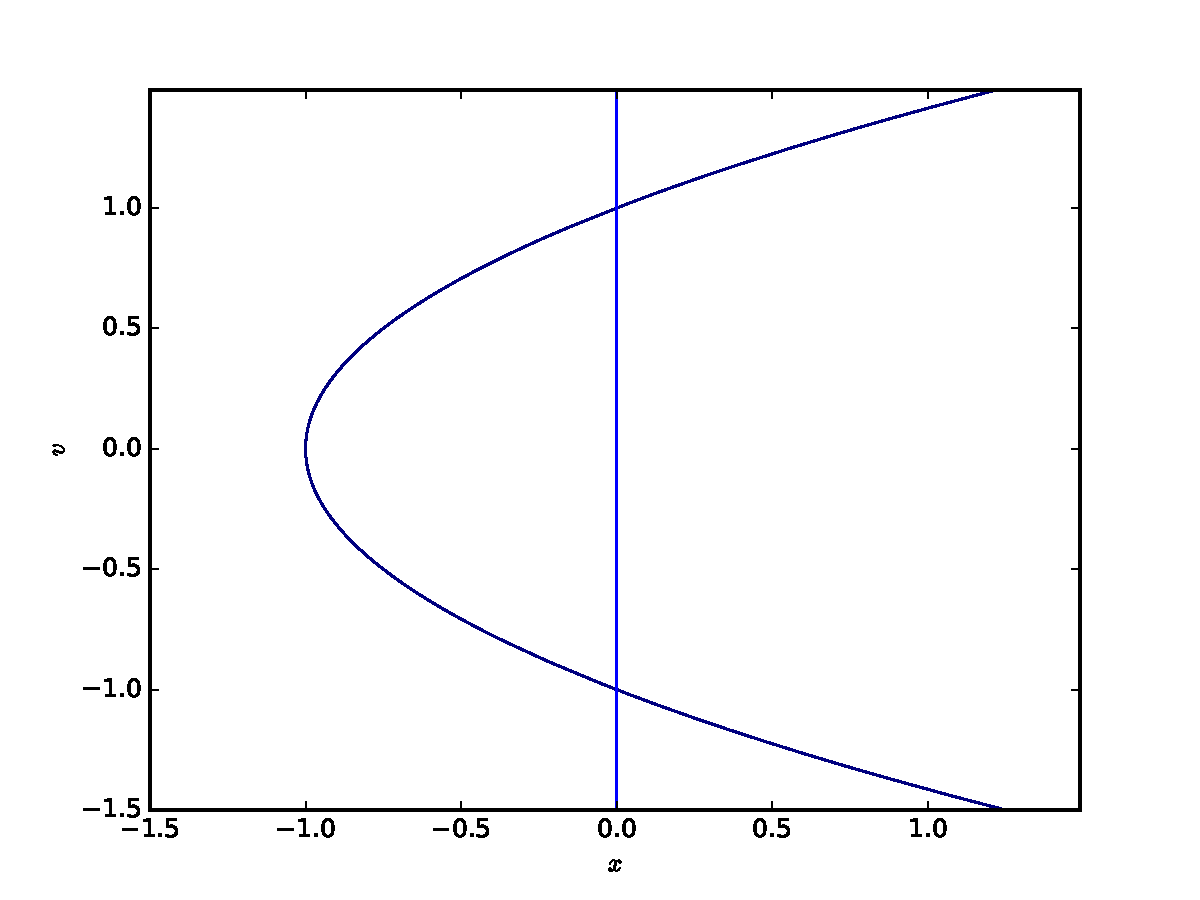
\includegraphics[width=1.1\textwidth]{pictures/node_affine_1.pdf}
                \caption{The affine chart resulting from setting $u = 1$ and
                eliminating $y$ in the original equation.}
            \end{subfigure}
            ~
            \begin{subfigure}[t]{0.4\textwidth}
                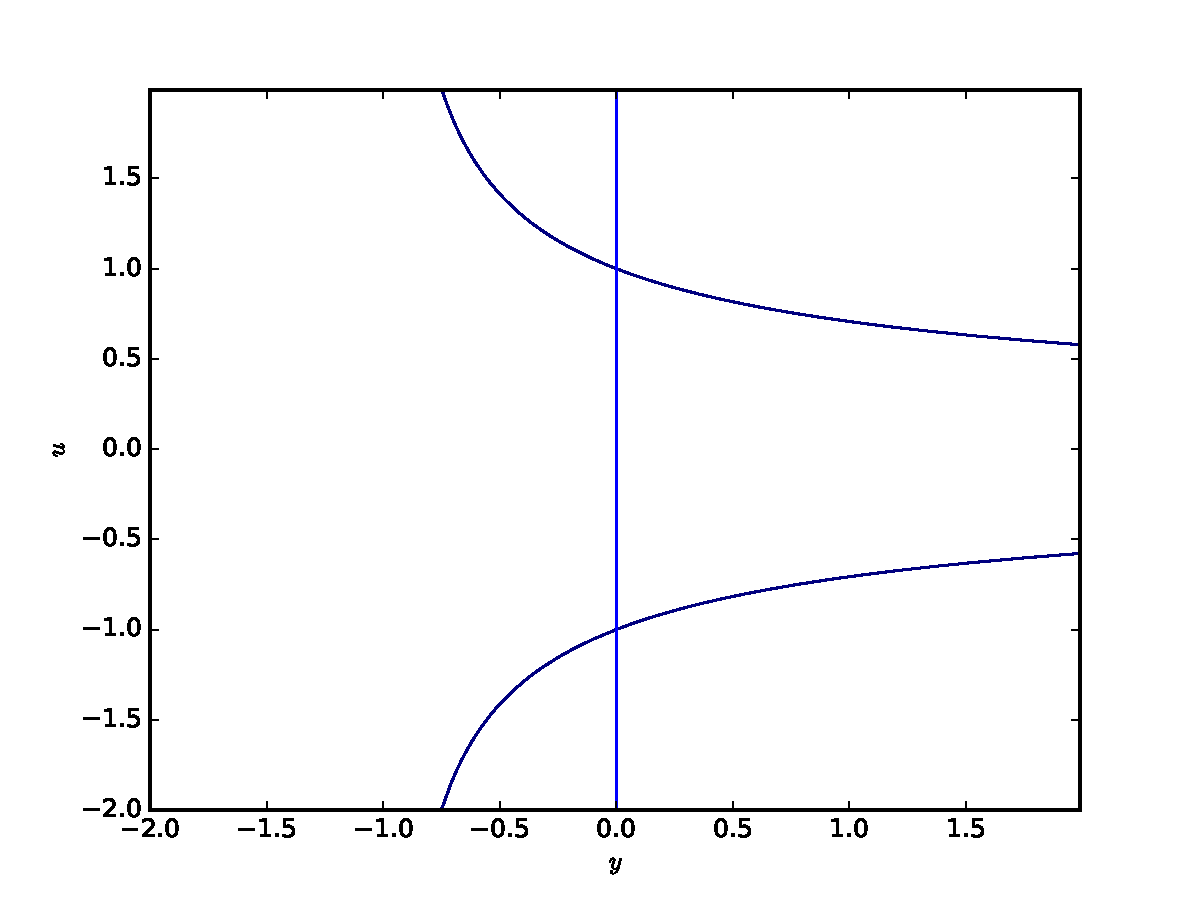
\includegraphics[width=1.1\textwidth]{pictures/node_affine_2.pdf}
                \caption{The affine chart resulting from setting $v = 1$ and
                eliminating $x$ in the original equation}
            \end{subfigure}
            \begin{subfigure}[t]{0.4\textwidth}
                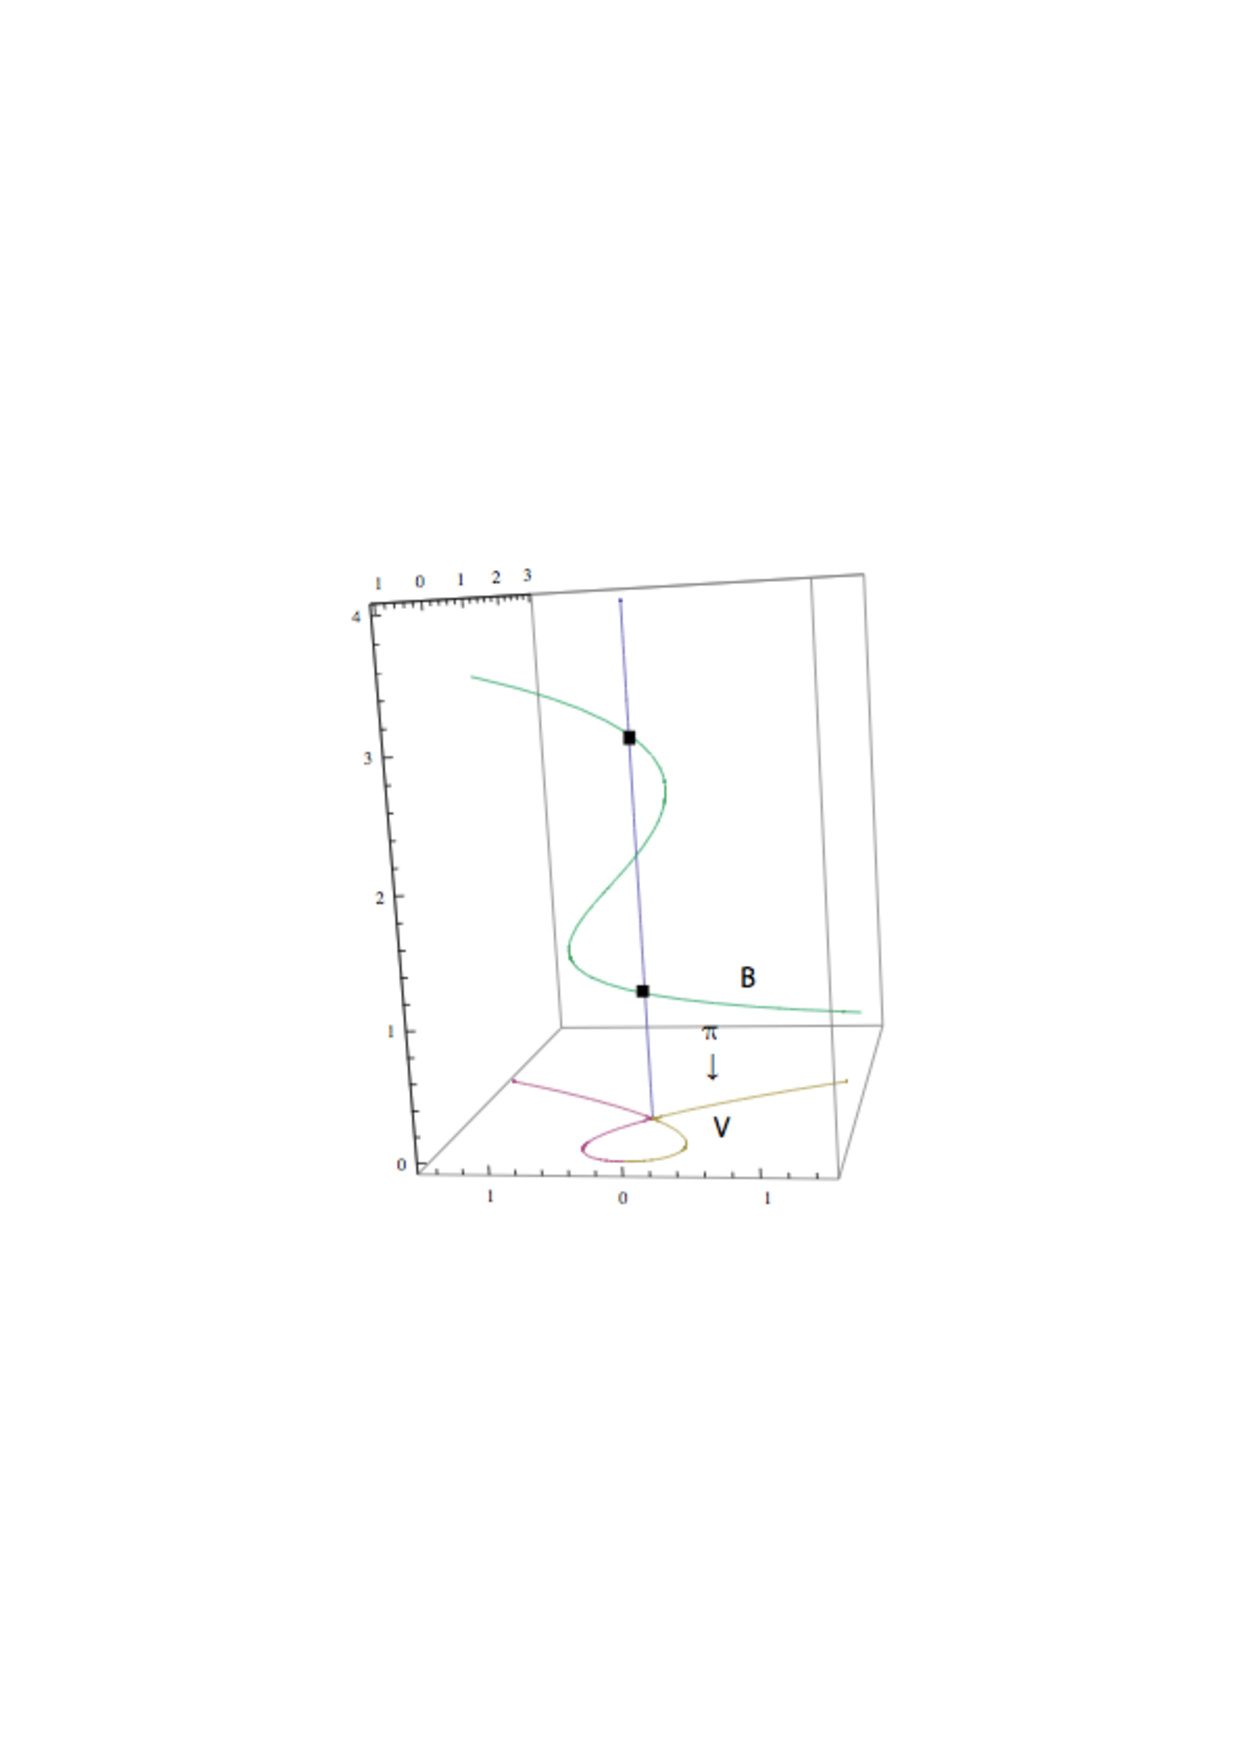
\includegraphics[width=1.0\textwidth]{pictures/blow_up_intuitive.pdf}
                \caption{A visual depiction of the blowup surface that clearly
                    shows how the singularity in the origin is resolved. Taken
                from \cite{Whi08}.}
                \label{fig:blow_up_intuitive}
            \end{subfigure}
            \caption{The affine charts of the Node. The vertical line plotted
                in slightly brighter blue, is called the \emph{exceptional
                divisor}\index{exceptional divisor} and corresponds to the
                blowup of what was the origin in the original surface. Note
                that the curves intersect the exceptional divisor in exactly
                two points. This corresponds to the double point singularity in the
                original surface.}
            \label{fig:affine_charts_node}
        \end{figure}
    \end{example}
    
    Blowing up singular surfaces or curves can be great fun and a lot of
    interesting pictures arise. We now take a look at an example where blowing
    up the surface in a single point is not sufficient for removing the
    singularities. 
    
    \subsection{Blowing up a line of singularity.}
    \label{sub:blowing_up_a_line_of_singularity_}
    
    In this section we will consider the algebraic surface 
    
    \clearpage
    \printbibliography \printindex
\end{document}

